\documentclass{article}

% if you need to pass options to natbib, use, e.g.:
%     \PassOptionsToPackage{numbers, compress}{natbib}
% before loading neurips_2021

% ready for submission
% \usepackage{neurips_2021}

% to compile a preprint version, e.g., for submission to arXiv, add add the
% [preprint] option:
% \usepackage[preprint]{neurips_2021}

% to compile a camera-ready version, add the [final] option, e.g.:
%     \usepackage[final]{neurips_2021}

% to avoid loading the natbib package, add option nonatbib:
\usepackage[nonatbib,preprint]{neurips_2021}

\usepackage[utf8]{inputenc} % allow utf-8 input
\usepackage[T1]{fontenc}    % use 8-bit T1 fonts
\usepackage{hyperref}       % hyperlinks
\usepackage{url}            % simple URL typesetting
\usepackage{booktabs}       % professional-quality tables
\usepackage{amsfonts}       % blackboard math symbols
\usepackage{nicefrac}       % compact symbols for 1/2, etc.
\usepackage{microtype}      % microtypography
\usepackage{xcolor}         % colors
\usepackage{graphicx}
\usepackage[numbers]{natbib}

\title{Research Proposal: An Agentic Framework for Synthetic Data Generation for
Fine-Tuning}

% The \author macro works with any number of authors. There are two commands
% used to separate the names and addresses of multiple authors: \And and \AND.
%
% Using \And between authors leaves it to LaTeX to determine where to break the
% lines. Using \AND forces a line break at that point. So, if LaTeX puts 3 of 4
% authors names on the first line, and the last on the second line, try using
% \AND instead of \And before the third author name.

\author{%
  Zachary Grannan \\
  \And{}
  Owen Ren
}

\begin{document}

\maketitle

\begin{abstract}
Synthetic data is now commonly used in the post-training stages of LLM
development. However, there has been less research into the use of
domain-specific synthetic data for fine-tuning purpose-built LLMs. For this
project, we propose the development of an open-source agentic framework, in the
style of AgentInstruct \citep{mitra_agentinstruct_2024}, that can automatically
generate synthetic data for LLM fine-tuning in particular domains. We will
evaluate the performance of LLMs developed via our framework compared to that of
traditional RAG-based approaches.
\end{abstract}

\section{Introduction}
Many commercial applications of large language models (LLMs) involve applying them to solve domain-specific tasks. Often, such applications require that additional domain-specific information, in particular information outside of the LLM training data, is made available to the LLM.

Retrieval-augmented generation (RAG) \citep{lewis_retrieval-augmented_2020} is a
popular technique for making such information available. In RAG, the application
injects data (e.g. from a database) into the system prompt, with the hope that
the LLM can use this information to produce a response that incorporates
relevant domain-specific data. An advantage of the RAG-based approach is its
flexibility and ease-of-use: the application can use its own logic to determine
how to enhance the prompts. However, RAG systems have corresponding
disadvantages. In particular, incorporating a RAG architecture increases
application and infrastructure complexity.

Fine-tuning presents another approach. In the fine-tuning paradigm, the parameters of the LLM itself are modified by training the LLM on additional content. The fine-tuned LLM can be used as a "drop-in" replacement for a base language model: no changes to architecture or software are required.

In prior work, various recipes have been proposed for developing specialized LLMs via fine-tuning \citep{balaguer_rag_2024,yang_fingpt_2023,wu_pmc-llama_2023}. Simultaneously, various techniques have been developed to improve general reasoning abilities with synthetic data \citep{shao_synthetic_2023,wang_self-instruct_2023,mitra_agentinstruct_2024}.

However, there is relatively less literature evaluating the performance of
state-of-the-art synthetic data generation techniques for fine-tuning
domain-specific LLMs. AgentInstruct \citep{mitra_agentinstruct_2024} provides a promising
agent-based approach, however the authors did not perform any evaluation for
domains-specific cases, and the AgentInstruct code is not readily available.

For this project, we propose the development of an open-source agentic framework
(in the style of AgentInstruct) that can automatically generate synthetic data
and fine-tune an LLM on that data. Concretely, we wish to make the following
contributions:

\begin{enumerate}
\item The development of the aforementioned framework
\item An evaluation that compares the performance of LLMs fine-tuned via our framework to traditional RAG based techniques
\item Reproducible experiments that track resource usage and the ability to leverage different language models
\end{enumerate}

\section{Related Work}

With the rapid advancements of new large language models (LLMs), there is
concern that the amount of internet data that has traditionally been used to
train these models has been exhausted. Recent releases of the latest models
have used synthetic data during pre- and post-training \citep{abdin_phi-3_2024,
dubey_llama_2024, bai_qwen_2023}. Furthermore, the generative and reasoning
capabilities of LLMs have proven their effectiveness as tools for synthetic data
generation.

\subsection{Fine-Tuning with Synthetic Data}

Recent research into leveraging LLMs for synthetic data generation is split
into two approaches: seeded methods where LLMs are guided by an initial dataset
to generate new data and seedless methods where LLMs generate data without an
initial dataset. In Self-Instruct \citep{wang_self-instruct_2023}, the authors
leverage vanilla GPT-3 to generate instructions, input, and output samples to
fine-tune the same language model, demonstrating a 33\% improvement over the
original model. In Synthetic Prompting \cite{shao_synthetic_2023}, they leverage
an LLM to generate Chain-of-Thought prompts to enhance a language model’s
reasoning capabilities during inference. In TarGEN \citep{gupta2023targen}, the
authors present a seedless multi-step prompting strategy that generates
high-quality synthetic datasets using LLMs, including on domain-specific tasks
with minimal existing data. Recent approaches to using LLMs for synthetic data
generation have led to agentic approaches that generate large amounts of diverse
and high-quality data. In AgentInstruct \citep{mitra_agentinstruct_2024}, seed
data is leveraged to transform and generate new data using curated LLM agents
across 17 different skills ranging from reading comprehension, question
answering, creative writing to few-shot reasoning. The resulting fine-tuned
Orca-3 model trained on the 22 million instructions generated from AgentInstruct
outperforms GPT-3.5-turbo and GPT-4 in the MMLU and DROP benchmarks.

\subsection{Integrating Knowledge Retrieval and Fine-Tuning}

Recent literature in combining fine-tuning with RAG, RAFT \citep{zhang2024raft},
has shown improvements in performance across domain-specific datasets. REALM
\citep{guu_realm_2020} augments a language model with a neural knowledge
retrieval engine that is also trained during the pre-training and fine-tuning
stages.

\subsection{Efficient Fine-Tuning}

Advancements in both fine-tuning, in which an existing model’s weights are used
as the baseline for further training, and improvements in small language models
have drastically reduced the computation required to fine-tune a model. Methods
like LoRA \citep{hu2021lora} and QLoRA \cite{dettmers2024qlora} have further
reduced the computation requirements for LLM finetuning.

While Large Language Models have significantly advanced natural language
processing, small language models (SLM) have also seen improvements in text
generation, reasoning, and performance. Training techniques such as model
distillation use an LLM to fine-tune an SLM, transferring knowledge from the LLM
to the SLM. Furthermore, SLMs have advantages in cost, computation, and
flexibility over LLMs. While LLMs excel at generalisability, recent research has
shown that SLMs fine-tuned on domain-specific datasets can outperform
general-purpose LLMs for specific tasks.

\subsection{Domain-Specific LLMs}

Domain-specific LLMs, both those trained from scratch and those that fine-tune
an existing model, have been shown to outperform general-purpose LLMs. In the
former category, the closed-source BloombergGPT \citep{wu_bloomberggpt_2023},
trained from scratch on a dataset consisting of domain-specific and general
data, outperforms general-purpose LLMs on finance-related tasks.

Because training an LLM from scratch is extremely resource-intensive, approaches
based on fine-tuning are often more economically feasible. Such approaches
typically fine-tune an LLM by injecting additional knowledge and performing
instruction-tuning \citep{ouyang_training_2022}. FinGPT \citep{yang_fingpt_2023}
provides a framework for fine-tuning LLMs for finance-related tasks. The
lightweight model PMC-LLaMa \citep{wu_pmc-llama_2023} is developed by
fine-tuning a LLaMA model, and can outperform ChatGPT on various medical QA
tasks.

\section{Methodology}

\begin{figure}[h]
  \centering
  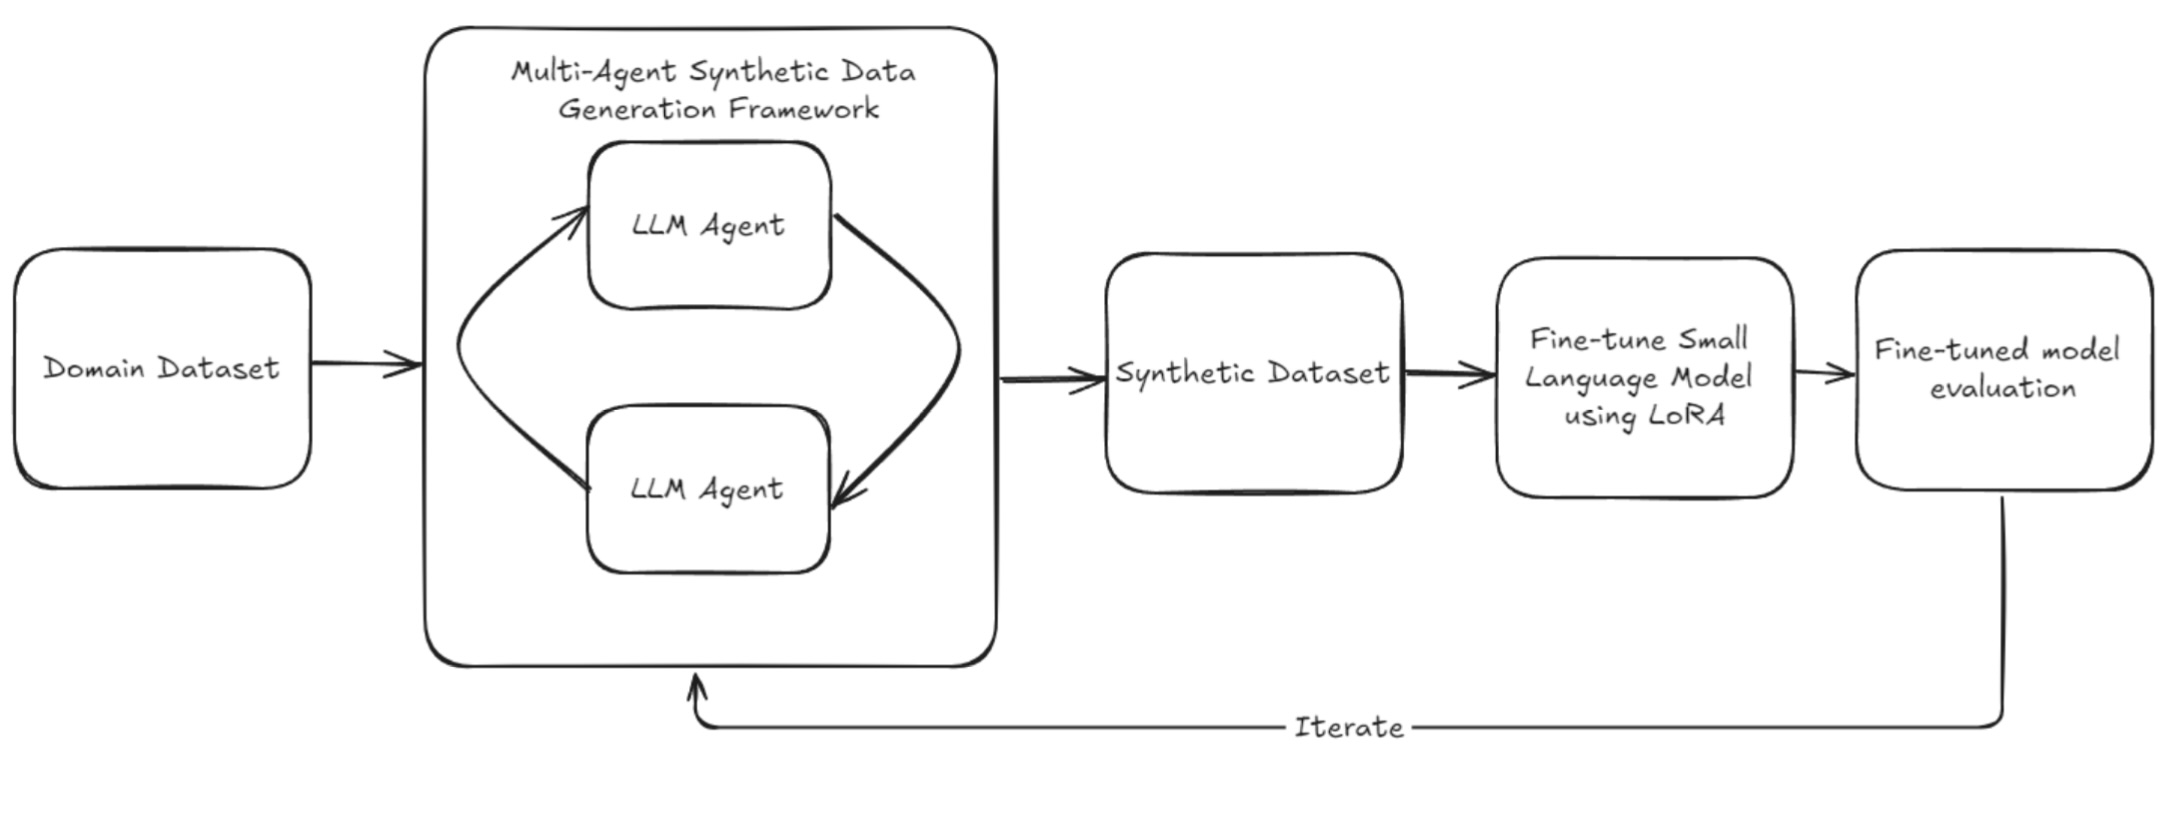
\includegraphics[width=1\textwidth]{methodology.jpg}
  \caption{An overview of our methodology. TODO}
\end{figure}

For our domain datasets that will be used as the seed data, we are still currently exploring datasets that can be used. Current ideas include research papers, company financial data, technical reports and manuals, or company specific FAQ data.
We will develop a multi agent synthetic data generation framework using small language models such as Llama-3.1-8B, Llama-3.2-3B, Qwen2.5-7B to synthetically generate high-quality diverse domain specific data.. Our immediate goal will be to create a framework for specializing in question answering tasks, similar to that of a traditional chatbot. Time permitting, we may expand this scope to also minimize hallucinations from model responses.
Next we will use the data to fine-tune LoRA adapters on the base model chosen. Since this will be an iterative process, we may also choose to perform a full supervised fine-tune of the model depending on resource limitations.

\subsection{Challenges}

One of the challenges we foresee may be overfitting on the fine-tuned model and the models inability to generalize to different writing styles and formats. We plan to mitigate this by increasing the diversity of our generated data. Another challenge is hallucination: previous research has shown that fine-tuning LLMs with new factual information increases their tendency to hallucinate (Gekhman et al. 2024). However, because we consider applications where the questions posed to the LLMs are related to data in the fine-tuning dataset, it's possible that this effect will be reduced (as opposed to questions unrelated to the domain, where a clear effect has already been observed in existing literature).

\section{Evaluation}
We will evaluate our approach with respect to two research questions:

\begin{itemize}
\item RQ1: How does our approach compare to RAG-based approach w.r.t. QA tasks?
\item RQ2: How does our approach compare to RAG-based approach w.r.t. hallucinations?
\end{itemize}

To evaluate performance, we will compare responses on a curated test dataset
against a baseline retrieval-augmented generation system and evaluate the
responses using an oracle model: previous research has shown that LLMs are
effective at approximating human preferences related to chatbot output
\citep{zheng_judging_2023}. We will leverage existing tools such as Ragas
\citep{ragas} for evaluation.

For our evaluation, we intend to consider existing off-the-shelf evaluation
suites. For example, we could consider one of the following domain-specific QA
benchmarks:

\begin{itemize}
\item TriviaQA \citep{joshi_triviaqa_2017} - A dataset consisting of 650k question-answer-evidence triples, sourced from trivia enthusiasts.
\item HotpotQA \citep{yang_hotpotqa_2018} - Contains 113K question-answer pairs from Wikipedia, alongside supporting evidence.
\item PubmedQA \citep{jin_pubmedqa_2019} - Nearly 300k QA instances derived from PubMed abstracts. Each instance takes the form of a research question with possible answers yes/no/maybe.
\end{itemize}

During our evaluation, we will fine-tune existing open-source models such as
Phi-3 \citep{abdin_phi-3_2024} and Llama 3 \citep{dubey_llama_2024}, etc. Resource permitting,
we will perform our approach on different sizes (e.g., for the Phi-3 series, 3.8B,
7B, and 14B models are available), considering how the different models perform
for RAG and fine-tuning approaches. We will also consider different quantization
levels.

\section{Conclusion}

In this work, we developed an agentic framework for synthetically generating
fine-tuning data. We evaluated our approach by creating a synthetic data
generation pipeline for answering QA tasks, and comparing its performance
against a RAG-based approach. Our results suggest that models finetuned using
our framework can achieve comparable performance compared to the RAG-based
approach.

As future work, we could consider evaluating our approach to generate finetuned
models for additional datasets to determine whether our technique applicable
across a range of domains. Additionally, there are several improvements we could
make to our "LLM-As-Judge" framework. In particular, enabling the judge to
return a numerical outcome to compare answer quality may yield more accurate
results compared to the current implementation which returns a binary decision.

\section{Threats to Validity}

Limitations related to time and computational resources result in a threat to external validity: we intend to use a NVIDIA 3080 TI GPU and compute resources from Google Colab for LLM fine-tuning, but in principle other organizations could extend significantly more resources towards LLM fine-tuning and consequently achieve better performance. Therefore, the results we observe may not be representative of what would be expected with the application of more computational resources.
One threat to internal validity is that the baseline RAG system that we develop for comparison purposes may itself have problems. To attempt to address this threat, we will try to the best of our ability to follow best practices in development of the RAG system to reduce the possibility of introducing bugs. We will also manually inspect the results of the RAG system to ensure that it is functioning properly.
The use of "LLM-as-judge" introduces a potential threat to construct validity: the oracle LLM itself may not be an accurate judge of the factual accuracy of answers. To address this threat, in our evaluation we will also judge a random subset of answers ourselves and ensure that they correspond with the oracle judgment to an acceptable level.


\clearpage

\bibliographystyle{abbrvnat}
\bibliography{bib}

\end{document}
